\section{CHESS - Lucas Weber}


\begin{frame}
	\frametitle{What is CHESS?}
	\begin{columns}
		\begin{column}{0.5\textwidth}
			\begin{itemize}
				\item \textbf{C}lassification of \textbf{He}terogenous \textbf{S}ensor \textbf{S}ignals\footnotemark
				\item Exploratory graph approach to a real-world sensor mapping problem (SIEMENS power plants)
				\item Deals with a wide variety of sensor signals and tries to map those to labels used for digital twins and simulations
			\end{itemize}
		\end{column}
		\begin{column}{0.45\textwidth}
			\vspace*{-3em}
			\begin{flushright}
				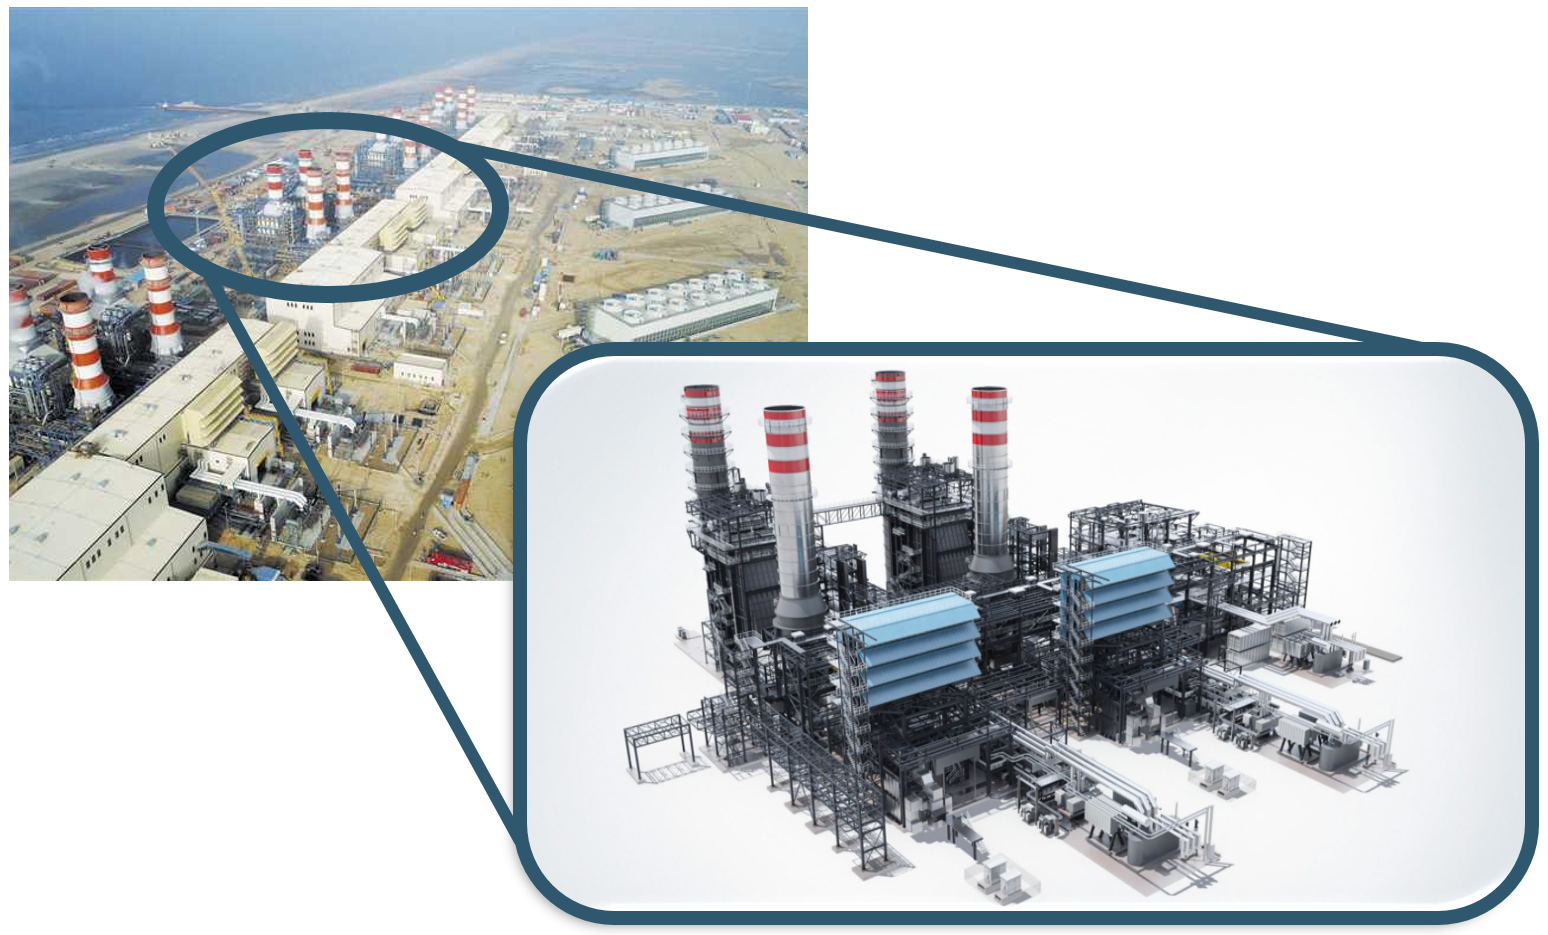
\includegraphics[width=0.8\textwidth]{img/research/PowerPlant.png}
				\begin{center}
					
\includegraphics[width=0.4\textwidth]{img/research/SElogo.png}
				\end{center}
			\end{flushright}
		\end{column}
	\end{columns}
	\footnotetext{Still working on that acronym though.}
\end{frame}

\begin{frame}
	\frametitle{What is the framework?}
	\begin{columns}
		\begin{column}{0.6\textwidth}
			\begin{itemize}
				\item We build a formal, directed and acyclic graph of algorithms to explore unknown sets of time series
				\item The problems are mainly in the context of time series processing, pattern detection and machine learning
				\item There are several open problems, where I could use the help of talented students
				\item \textbf{If you are interested, contact me. Most topics can be done as thesis, project work or as a student assistant!}
			\end{itemize}
		\end{column}
		\begin{column}{0.4\textwidth}
			\begin{center}
				\vspace*{-5em}
				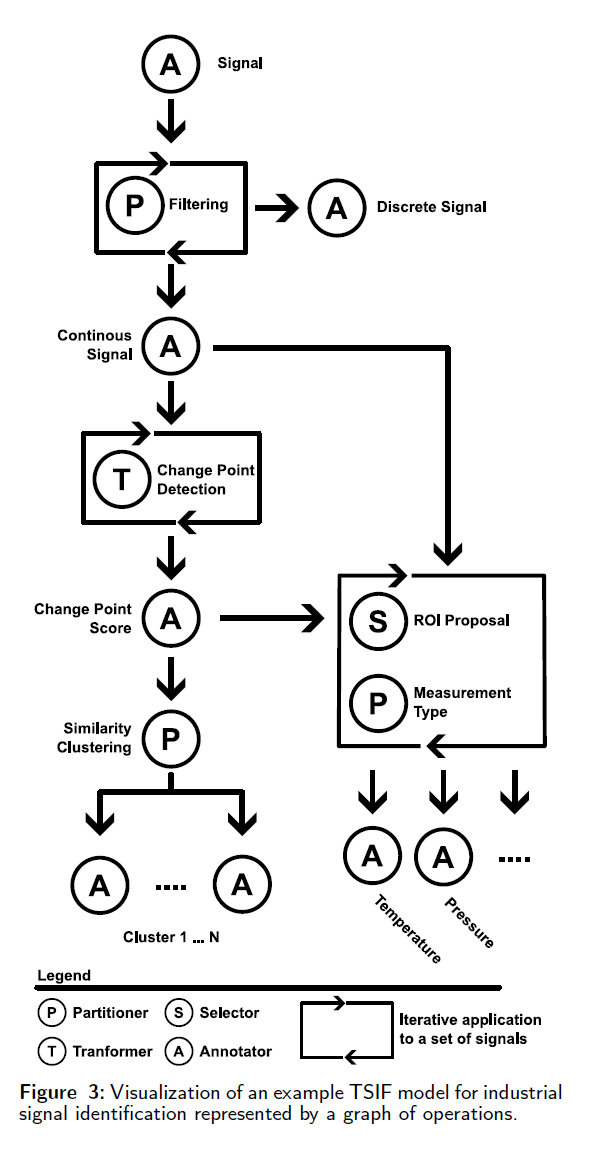
\includegraphics[height=\textheight]{img/research/ExampleGraph.png}
			\end{center}
		\end{column}
	\end{columns}
\end{frame}

\begin{frame}
	\frametitle{How can you contribute?}
	\begin{columns}
		\begin{column}{0.4\textwidth}
			\begin{center}
				\vspace*{-3em}
				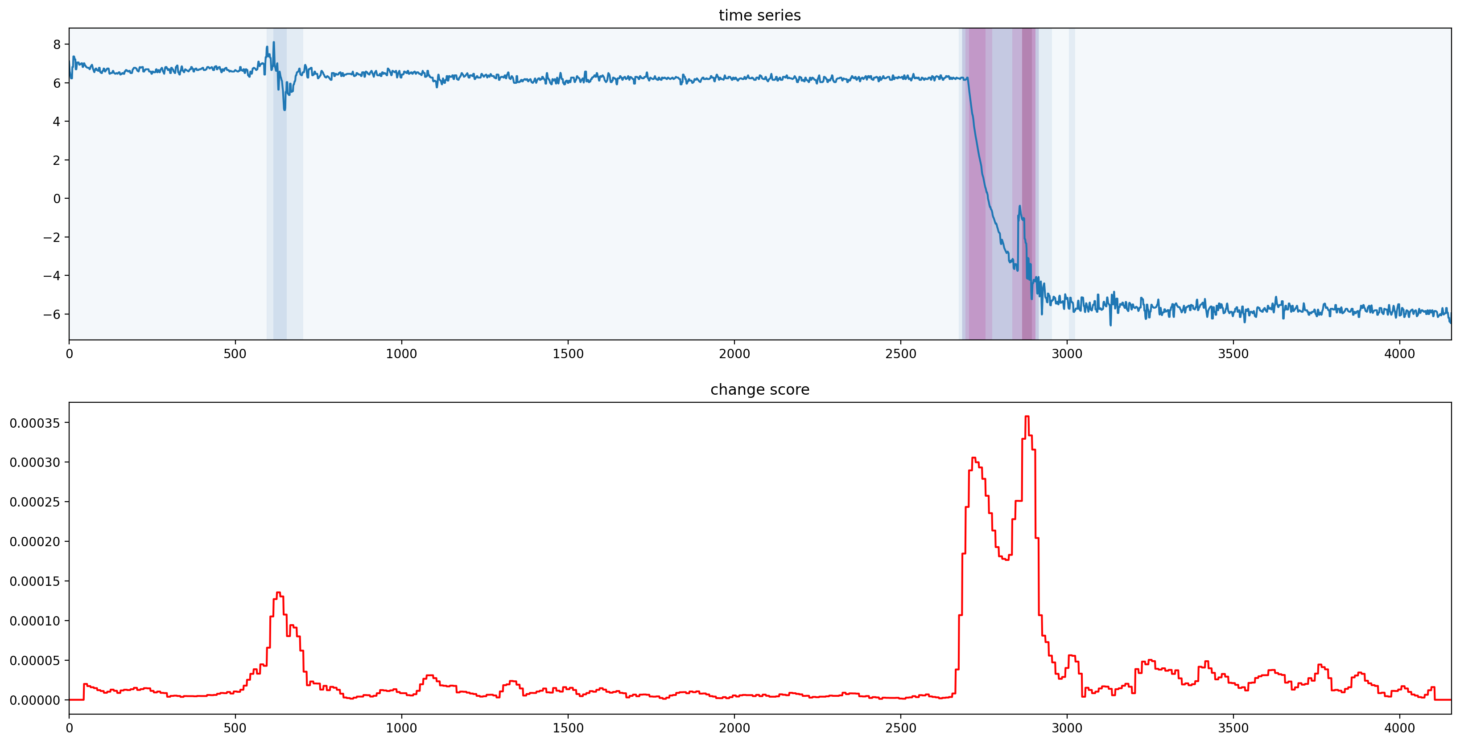
\includegraphics[width=\textwidth]{img/research/changepoint1.png}
				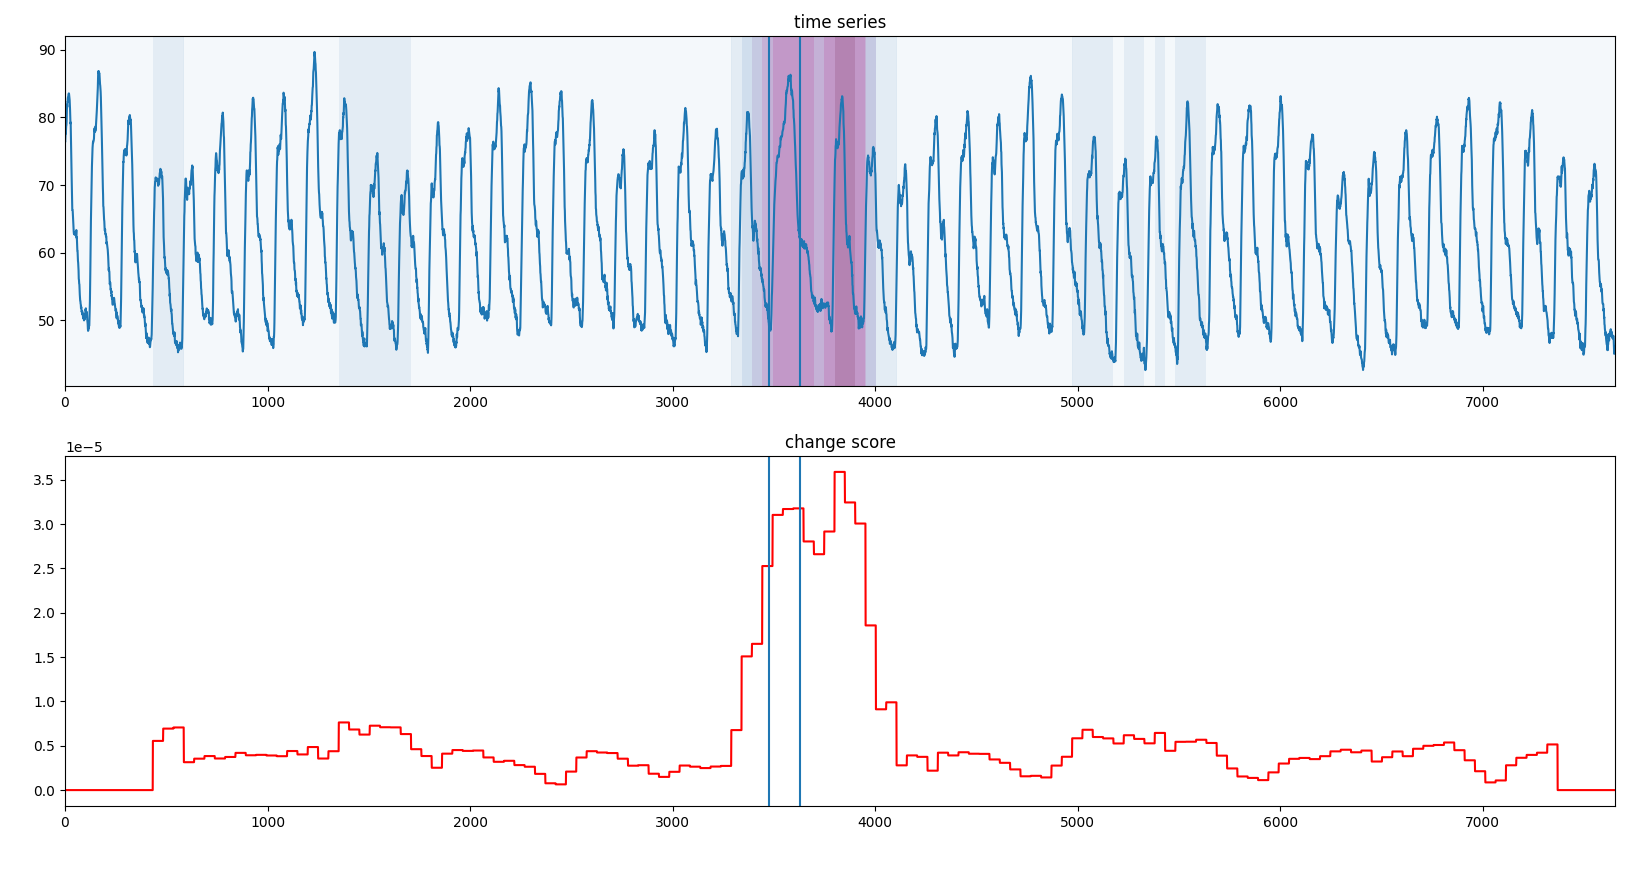
\includegraphics[width=1.01\textwidth]{img/research/changepoint2.png}
			\end{center}
		\end{column}
		\begin{column}{0.5\textwidth}
			\textbf{Find more information on my personal page!\footnotemark}
			\\
			Currently there are the following open topics:
			\begin{itemize}
				\item Change Point Correlation for Knowledge Discovery in Time Series Datasets (Device Detection, Botnet detection)
				\item Unit-free classification of sensor signals from power plants (Classical machine learning and siamese neural networks)
				\item Memory aware implementation of dynamic time warping in a low level language (e.g. Rust, C, C++)
				\item Architecture and Implementation of Change Point Detection Testbench
			\end{itemize}
		\end{column}
	\end{columns}
	\footnotetext{Check the github: https://github.com/Lucew/changepoynt and my personal page: https://www.cs6.tf.fau.de/person/lucas-weber/}
\end{frame}
\begin{frame}
	\frametitle{Let's look at some Results}
	\begin{columns}
		\begin{column}{0.4\textwidth}
			\begin{center}
				\vspace*{-3em}
				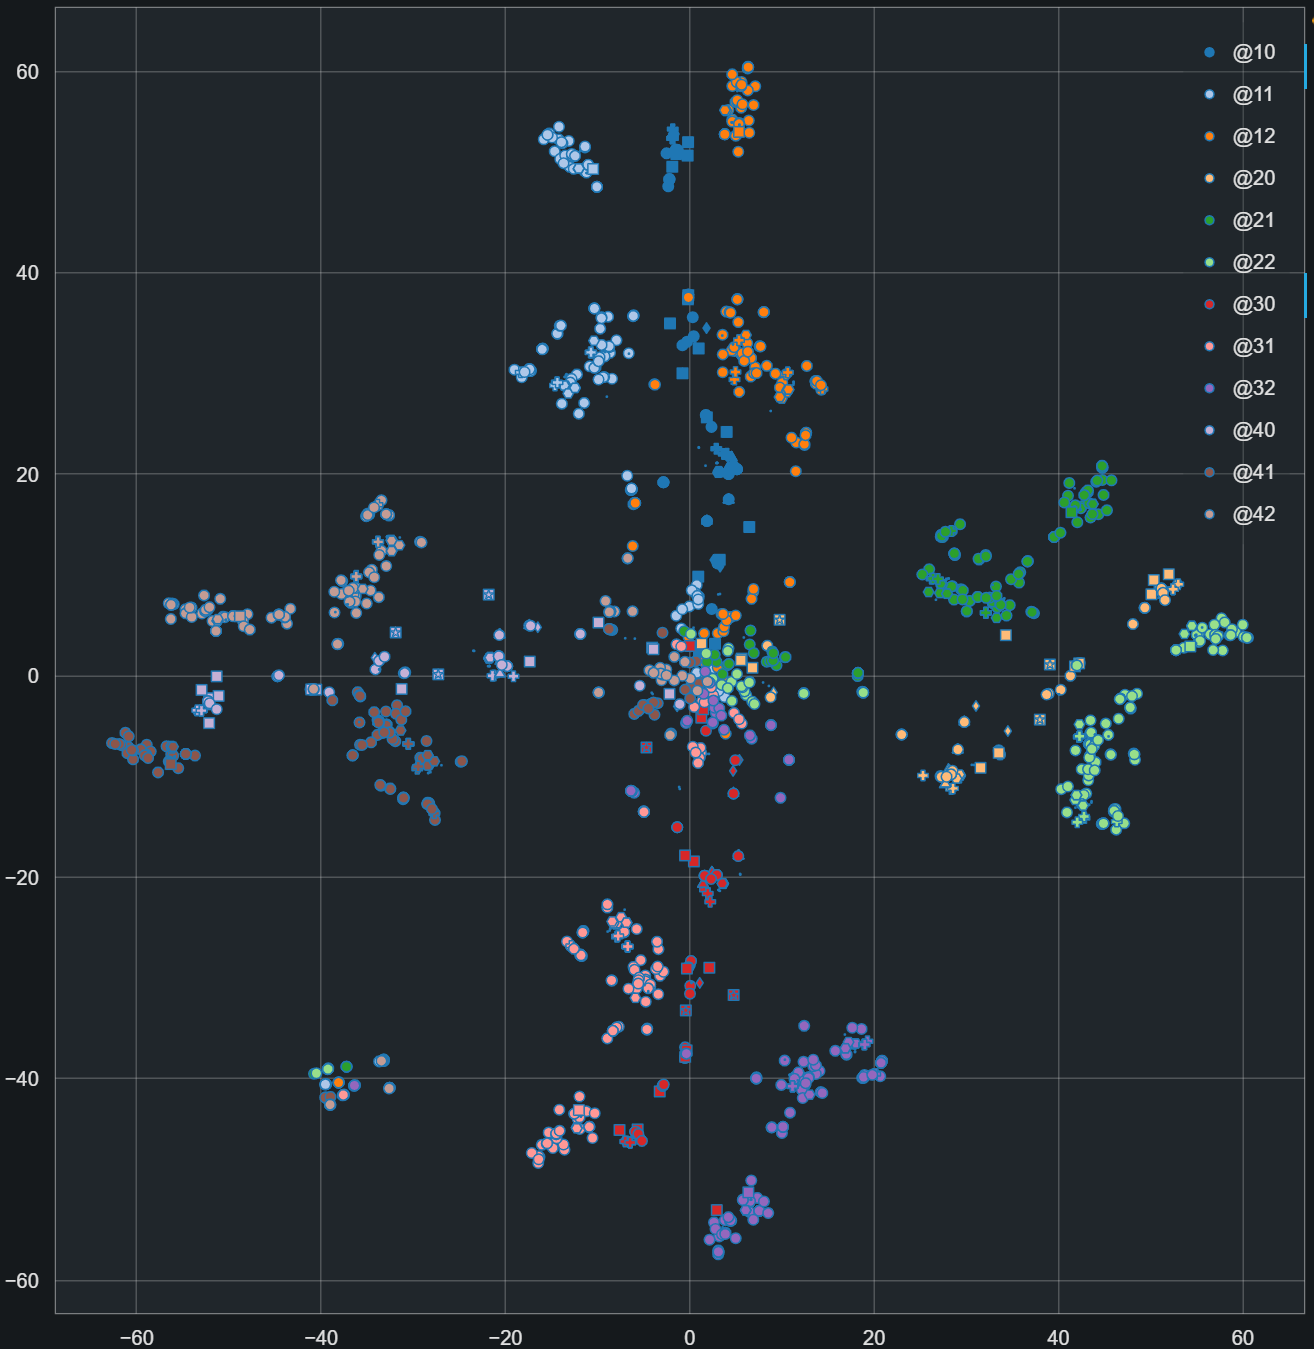
\includegraphics[width=\textwidth]{img/research/ChangePointClustering.png}
			\end{center}
		\end{column}
		\begin{column}{0.5\textwidth}
			\begin{center}
				\vspace*{-3em}
				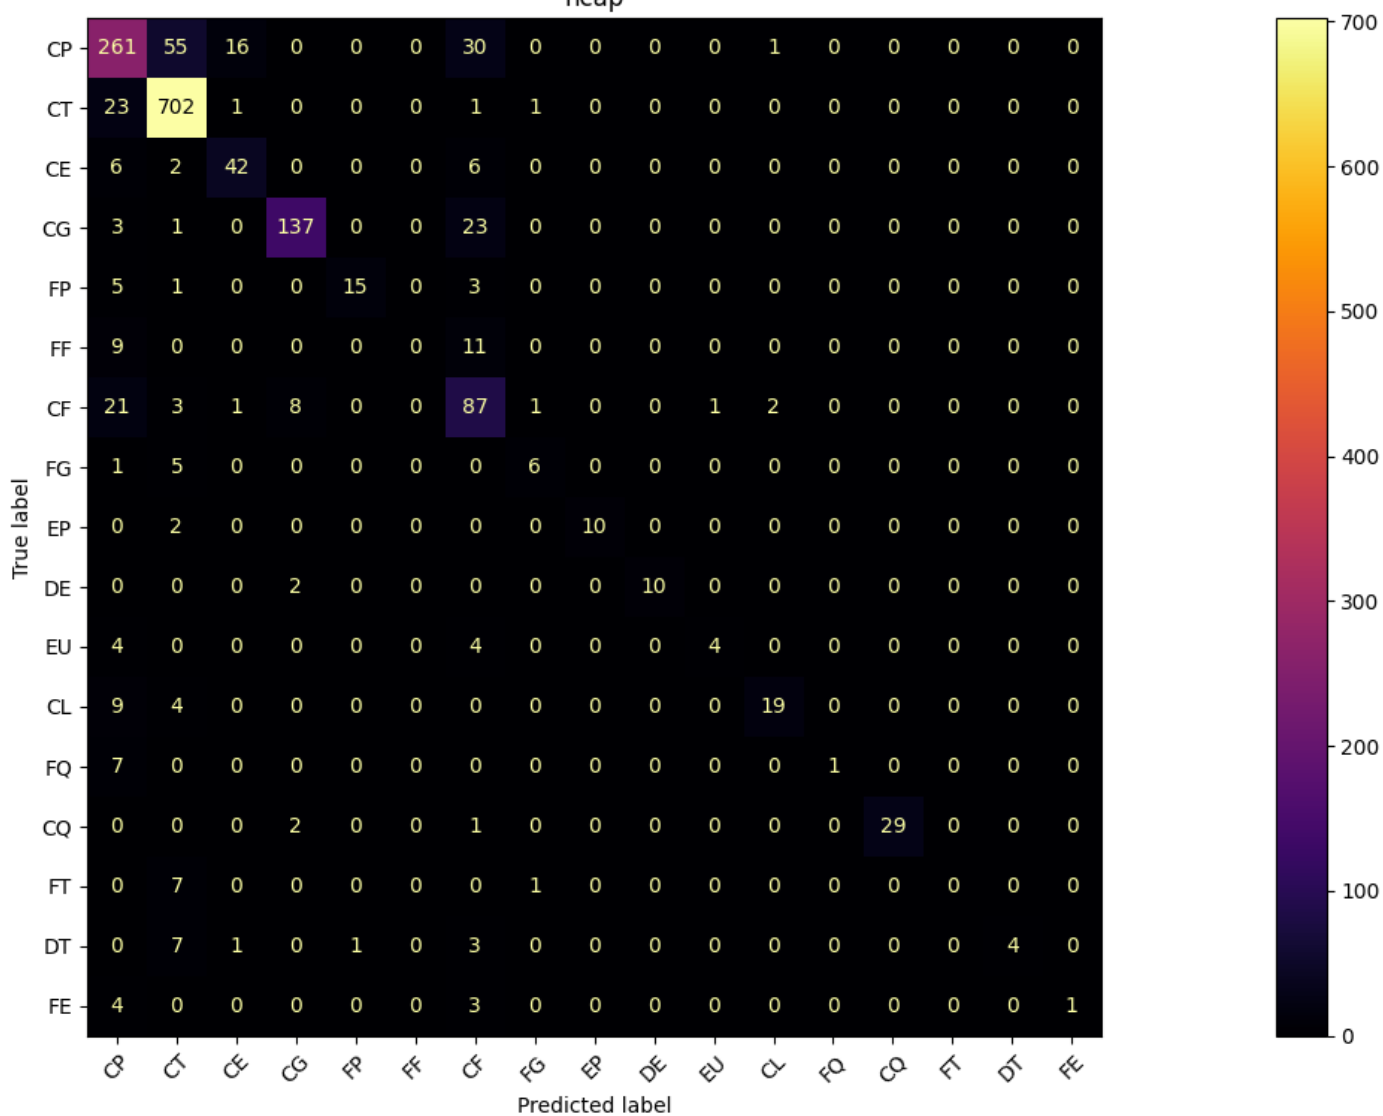
\includegraphics[width=\textwidth]{img/research/MeasurementMatrix.png}
			\end{center}
		\end{column}
	\end{columns}
\end{frame}
